\input{../head.tex}
\section{Identification polynômiale et étude mathématique}

Cette section a pour but d'expliquer notre démarche pour l'approximation de la fréquence de coupure
dans un circuit passe-bas et passe-haut. Trois méthodes nous étaient proposées, et nous avons adopté 
la première pour les raison explicitées plus bas.

Définissons tout d'abord ce qu'est la fréquence de coupure: c'est la fréquence à partir de laquelle 
la tension dans un circuit passe-bas (resp. passe-haut) commence à diminuer (resp. se stabiliser) 
lorsque la fréquence augmente.

Pour la déterminer, nous avons tout d'abord procédé à une expérience en laboratoire.
Celle-ci consistait à mesurer la tension de sortie en fonction de la fréquence du signal, et ce dans 
chacun des circuits considérés.
Graphiquement, le tracé du rapport des tensions d'entrée et de sortie des filtres en fonction de la 
fréquence a l'allure d'une exponentielle.  Pour faciliter le calcul, nous sommes passés en repère 
semi-logarithmique, réduisant ainsi l'exponentielle à une intersection de deux droites. Ce procédé
explicité en profondeur dans la sous-section "Passage en échelle logarithmique"'.

\subsection{Approximation de la fréquence de coupure}

\subsubsection{Filtre passe-bas}

\begin{figure}[ht!]
\centering
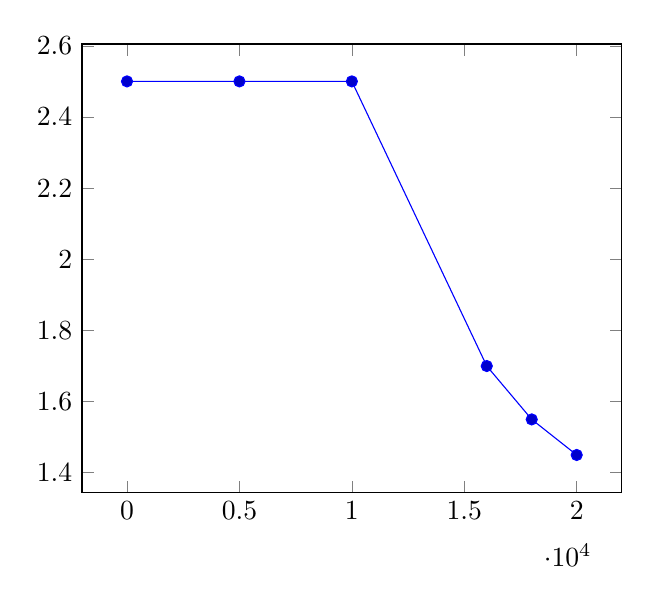
\begin{tikzpicture}
    \begin{axis}
\addplot coordinates
{(0,2.5) (5000,2.5) (10000,2.5) (16000,1.7) (18000,1.55) (20000,1.45)};
\end{axis}
\end{tikzpicture}
\caption{Graphe de $V_{out}$ expérimentale en fonction de la fréquence}
\label{lwp_ratio}
\end{figure}



\paragraph{Équation de la droite horizontale}
Expérimentalement, nous obtenons une fréquence de sortie constante (de $\unit{2.5}{\volt}$ ) 
pour les plus basses fréquences. L'équation de la droite horizontale est donc \[y=2.5\]

\paragraph{Équation de la droite diagonale}

Avec les mesures effectuées en laboratoires, nous n'obtenons non pas une droite mais bien une exponentielle. 
Pour faciliter le calcul de l'intersection de l'exponentielle et de la droite, nous passons donc en repère 
semi-logarithmique. 

Nous savons que l'équation d'une droite dans un repère cartésien est de type $y=ax+b$, avec $a$ la pente 
et $b$ l'ordonnée à l'origine.

Mais ici nous ne sommes plus dans un repère cartésien mais bien dans un répère semi-log selon l'axe des 
abscisses. L'équation de la droite devient alors : $y=a\log{x}+b$

\paragraph{Mesures en laboratoires}

Voici 3 résultats choisis de manière cohérente parmi toutes les mesures effectuées en laboratoire, où 
$V_c$ est la tension de sortie et $f$ la fréquence :

\begin{center}
\begin{tabular}{|c|c|c|}
\hline
$V_c$ & $f$ & $\log{f}$ \\
\hline
1.7 & 16000 & 4.204 \\
\hline
1.55 & 18000 & 4.255 \\
\hline
1.45 & 20000 & 4.301 \\
\hline
\end{tabular}
\end{center}

Dès maintenant, les fréquences sont exprimées en base logarithmique.
Écrivons un système ayant pour inconnues la pente ($a$) et l'ordonnée à l'origine ($b$) de notre droite 
inconnue.
Nous avons trois équations à deux inconnues, et le système n'admet pas de solution.
Cela n'est pas étonnant, étant donné que les résultats expérimentaux ne sont jamais très précis.

Voici le système sous forme matricielle :

$$A \cdot \vec{x} = \vec{b}$$

\begin{center}
\begin{array}{rcel}
$$
\begin{pmatrix}
4.204 & 1\\
4.255 & 1 \\
4.301 & 1
\end{pmatrix} &

\begin{pmatrix}
a\\
b
\end{pmatrix} &

= &

\begin{pmatrix}
1.7\\
1.55\\
1.45
\end{pmatrix}
$$
\end{array}
\end{center}	

Le système n'admet pas de solution car $\vec{b}$ n'appartient pas à l'espace des colonnes de $A$. Nous 
allons donc projeter $\vec{b}$ sur l'espace des colonnes de $A$ afin d'obtenir une solution approchée.

Soient $f_1$, $f_2$ les colonnes de $A$, et donc les éléments de la base de l'espace des colonnes de $A$.
Trouvons une base orthonormée $(e_1, e_2)$ de l'espace colonnes de la matrice en utilisant
la méthode de Gram-Schmidt :

$$e_1 = \frac{f_1}{||f_1||} = (\frac{1}{\sqrt{3}} ; \frac{1}{\sqrt{3}} ; \frac{1}{\sqrt{3}})$$

$$e_2 = \frac{f_2 - (e_1|f_2)}{||f_2 - (e_1|f_2)||} = (-0.684 ; 0.03 ; 0.729)$$


Nous sommes maintenant en mesure de trouver une projection du vecteur contenant nos données expérimentales
peu précises :
nous projetons les vecteurs grâce à la formule de la projection :

% Peut-être parler ici du fait qu'on projete plutôt sur A orthogonal pour gagner du temps en calcul ?

$$
b'
=
(b|e_1) \cdot e_1 + (b|e_2) \cdot e_2
=
\begin{pmatrix}
1.607\\
1.556\\
1.524
\end{pmatrix}$$
$$

Nous pouvons alors réécrire le système comme cela :

$$
\begin{pmatrix}
 4.204 & 1\\
 4.255 & 1 \\
 4.301 & 1
\end{pmatrix}
\begin{pmatrix}
a\\
b
\end{pmatrix}
=
\begin{pmatrix}
1.607\\
1.565\\
1.524
\end{pmatrix}
$$


Nous en déduisons la valeur des coefficients $a$ et $b$ :

$$a = -1.96$$
$$b= 9.84$$

La droite oblique a donc pour équation
$$\fbox{y= -1.96 \timeslog{x} +9.84}$$

Pour trouver la fréquence d'intersection entre les deux droites, nous résolvons le système, et nous
trouvons :

$$\fbox{x = \unit{5557.7}{\hertz}}$$

Cela nous semble correct car en théorie nous devions arriver à une valeur $f$ telle que :

$$f=\frac{1}{2\pi RC}$$

avec $R= 7.5 + 50 = \unit{57.5}{\ohm}$ et $C= \unit{470 \cdot 10^{-9}}{\farad}$, la valeur théorique de 
la fréquence de coupure est donc :

$$f= \unit{5889.2}{\hertz}$$

\subsubsection{Filtre passe-haut}

\begin{figure}[ht!]
\centering
\begin{tikzpicture}[>=stealth]
\begin{axis}[
axis x line=middle,
axis y line=middle,
axis line style=->,
xlabel={$f$},
ylabel={$V_{out}$},
]

\addplot coordinates
{(127,0.4) (191,0.5) (356,0.6) (600,0.75) (800,0.75) (1000, 0.75)};
\end{axis}
\end{tikzpicture}
\caption{Graphe de $V_{out}$ expérimentale en fonction de la fréquence}
\label{lwp_ratio}
\end{figure}
\paragraph{Équation de la droite horizontale}

Nous savons que l'équation de la droite horizontales est $y = 0.75$.

\paragraph{Équation de la droite diagonale}

Nous allons encore utiliser une base logarithmique pour la pente, pour les mêmes raison explicitées pour
le filtre passe-bas.
L'équation de la droite est donc de la forme : $y=a \log{x}+b$.

Voici 3 résultats choisis parmi les mesures effectuées en laboratoire :

\begin{center}
\begin{tabular}{|c|c|c|}
\hline
$V_c$ & $f$ & $\log{f}$ \\
\hline
0.4 & 127 & 2.1\\
\hline
0.5 & 191 & 2.3\\
\hline
0.6 & 356 & 2.6 \\
\hline
\end{tabular}
\end{center}

De manière analogue que pour le premier filtre, nous formons le système suivant :

\begin{center}
\begin{array}{rcel}
$$
\begin{pmatrix}
2.1 & 1\\
2.3 & 1 \\
2.6 & 1
\end{pmatrix}&

\begin{pmatrix}
a\\
b
\end{pmatrix}&

=&

\begin{pmatrix}
0.4\\
0.5\\
0.6
\end{pmatrix}
$$
\end{array}
\end{center}


Transformons maintenant la base quelconque $(f_1, f_2)$ de l'espace des
colonnes de $A$ en une base orthonormée $(e_1, e_2)$ afin de pouvoir
calculer la projection orthogonale ensuite :

$$e_1 = \frac{f_1}{||f_1||} = (\frac{1}{\sqrt{3}} ; \frac{1}{\sqrt{3}} ; \frac{1}{\sqrt{3}})$$

$$e_2 = \frac{f_2 - (e_1|f_2)}{||f_2 - (e_1|f_2)||} = (-0.6, 0, 0.8)$$

Et nous obtenons comme vecteur projeté $\vec{b}'$ :

$$
\begin{pmatrix}
0.36\\
0.5\\
0.69
\end{pmatrix}
$$

Nous pouvons alors réécrire le système comme ceci :

$$
 \begin{pmatrix}
  2.1 & 1\\
  2.3 & 1 \\
  2.6 & 1
 \end{pmatrix}
 \begin{pmatrix}
 a\\
 b
 \end{pmatrix}
 =
 \begin{pmatrix}
 0.36\\
 0.5\\
 0.69
 \end{pmatrix}
$$

Nous en déduisons la valeur des coefficients $a$ et $b$ :

$$a =0.7$$ 
$$b= -1.11$$

L'équation de la droite est alors :

$$ \fbox{y= 0.7 \log{x} - 1.11} $$

Pour trouver l'intersection entre les deux droites nous résolvons le système, et nous trouvons:

$$ x = \unit{439.4}{\hertz}$$

% wtf, ne concorde pas avec la valeur théorique...

\subsection{Choix de la méthode}

Une démarche d'approximation n'est évidemment pas unique. Nous avions le choix entre trois méthodes 
distinctes, et nous avons opté pour celle utilisant les bases orthonormées.
%todo

\subsection{Meilleure approximation}

Pour arriver à une meilleure approximation, nous pourrions imaginer considérer $n$ points avec un 
$n$ très grand. Cependant, ...
% todo

\subsection{Passage en échelle logarithmique}

Lors de notre approximation, nous avons mentionné le fait que nous "passions en échelle logarithmique". 
Généralement, nous utilisons des échelles linéaires, avec des graduations dont la différence est constante.
Ici, dans un soucis de facilité, nous avons utilisé une représentation semi-logarithmique. Cela signifie
que les graduations ont un rapport constant, et non plus une différence constante pour l'axe des abscisses.
Cela nous permet de travailler à grande échelle, et de représenter l'exponentielle comme une droite, de
manière simple. L'équation de la droite est, en toute généralité : $y=a\log{x}+b$ .

\end{document}

\input{../foot.tex}
